\documentclass{article}
\usepackage{tikz}
\usetikzlibrary{automata, positioning, arrows}
\usepackage[margin=1cm]{geometry}
\usepackage{caption}

\begin{document}


\section*{Zadanie 1}
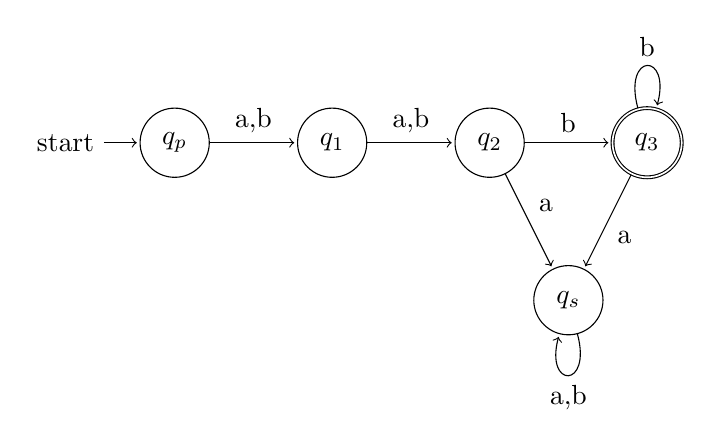
\begin{tikzpicture}[shorten >=1pt,node distance=2cm,on grid,auto]

    \node[state, initial] (q_p) {$q_p$};
    \node[state] (q_1) [right=of q_p] {$q_1$};
    \node[state] (q_2) [right=of q_1] {$q_2$};
    \node[state, accepting] (q_3) [right=of q_2] {$q_3$};
    \node[state] (q_s) [below right=2cm and 1cm of q_2] {$q_s$};

    \path[->]
    (q_p) edge node {a,b} (q_1)
    (q_1) edge node {a,b} (q_2)
    (q_2) edge node {b}   (q_3)
          edge node {a}   (q_s)
    (q_3) edge [loop above] node {b} ()
          edge node {a} (q_s)
    (q_s) edge [loop below] node {a,b} ();
    
\end{tikzpicture}

\section*{Zadanie 2}
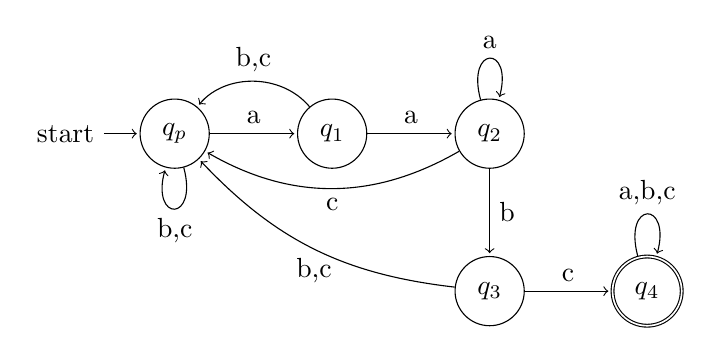
\begin{tikzpicture}[shorten >=1pt,node distance=2cm,on grid,auto]

    \node[state, initial] (q_p) {$q_p$};
    \node[state] (q_1) [right=of q_p] {$q_1$};
    \node[state] (q_2) [right=of q_1] {$q_2$};
    \node[state] (q_3) [below=of q_2] {$q_3$};
    \node[state, accepting] (q_4) [right=of q_3] {$q_4$};

    \path[->]
    (q_p) edge [loop below] node {b,c} ()
          edge node {a} (q_1)
    (q_1) edge [bend right=50] node [above] {b,c} (q_p)
          edge node {a} (q_2)
    (q_2) edge [loop above] node {a} ()
          edge node {b} (q_3)
          edge [bend left=30] node {c} (q_p)
    (q_3) edge node {c} (q_4)
          edge [bend left=20] node [below] {b,c} (q_p)
    (q_4) edge [loop above] node {a,b,c} ();

\end{tikzpicture}

\section*{Zadanie 3}
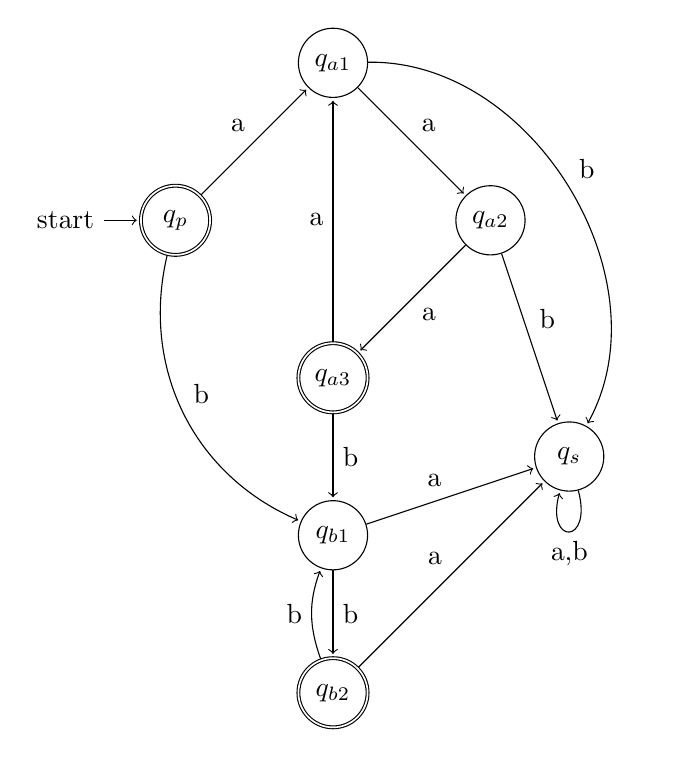
\begin{tikzpicture}[shorten >=1pt,node distance=2cm,on grid,auto]

    \node[state, initial, accepting] (q_p) {$q_p$};
    \node[state] (q_a1) [above right=2cm and 2cm of q_p] {$q_{a1}$};
    \node[state] (q_a2) [below right=2cm and 2cm of q_a1]{$q_{a2}$};
    \node[state, accepting] (q_a3) [below right=2cm and 2cm of q_p] {$q_{a3}$};
    \node[state] (q_b1) [below=of q_a3] {$q_{b1}$};
    \node[state, accepting] (q_b2) [below=of q_b1] {$q_{b2}$};
    \node[state] (q_s) [above right=1cm and 3cm of q_b1]{$q_s$};

    \path[->]
    (q_p) edge node {a} (q_a1)
          edge [bend right=40] node {b} (q_b1)
    (q_a1) edge node {a} (q_a2)
            edge [bend left=60] node {b} (q_s)
    (q_a2) edge node {a} (q_a3)
            edge node {b} (q_s)
    (q_a3) edge node {a} (q_a1)
            edge node {b} (q_b1)
    (q_b1) edge node {a} (q_s)
            edge node {b} (q_b2)
    (q_b2) edge node {a} (q_s)
            edge [bend left=20] node {b} (q_b1)
    (q_s) edge [loop below] node {a,b} ();
    
\end{tikzpicture}


\end{document}